\chapter{Simple Storage Service (S3)}\label{ch:simple-storage-service}

AWS S3 is a form of cloud-based object storage.
This is a style of network filesystem that treats each file as a separate object with a unique ID, which allows each
object to be served individually over a network with a single URL, which can also be enhanced with a content delivery
network~\parencite{amazon2022cloud}.

Each S3 instance is seperated into logical containers known as buckets.
Each S3 bucket can have its own credentials, its own endpoint and other permissions and configuration.
Object storage is particularly useful when creating an application that scales as you are billed per unit of storage
that you use, and in theory are able to use infinite storage as your application demands.
The only limitation with object storage is how much you are able to pay for.
Each object is automatically replicated across many nodes, providing data redundancy against multiple different
availability zones.

S3 is perhaps the most popular AWS service and used by many SaaS applications across the internet, for instance
Instagram, Facebook, Discord and Twitter are all known for using S3 or S3-style storage.
The advent of object storage has created an almost de-facto standard, which has lead for the creation of many
'S3-compatible' or 'S3-like' competitor solutions, such as those run by Google Cloud and Microsoft Azure.

\begin{figure}
    \centering
    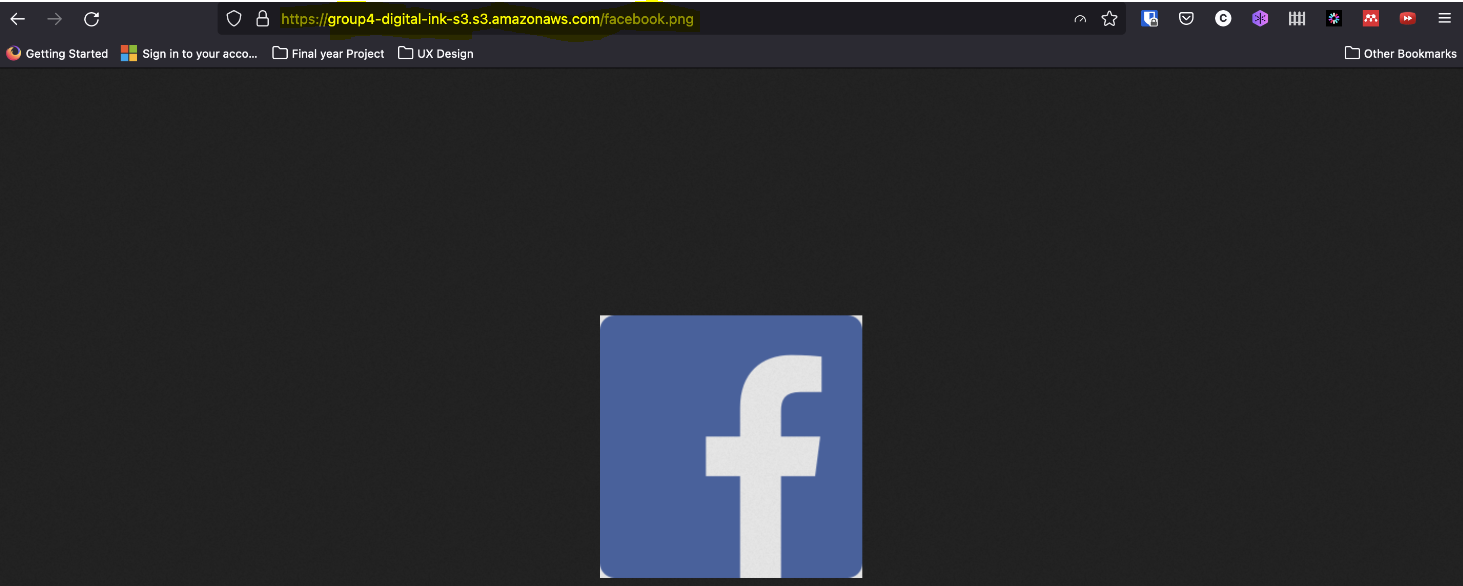
\includegraphics[width=\textwidth]{resources/s3/s3-image-displayed}
    \caption{Image access through S3.}
    \label{fig:s3-image}
\end{figure}

\begin{figure}
    \centering
    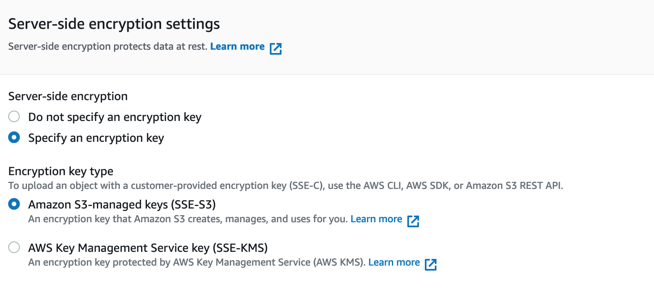
\includegraphics[width=\textwidth]{resources/s3/s3_encryption.PNG}
    \caption{Image access through S3.}
    \label{fig:s3-image-2}
\end{figure}